\documentclass[a4paper]{article}
\usepackage[utf8]{inputenc}
\usepackage[francais]{babel}
\usepackage[babel=true]{csquotes}
\usepackage{graphicx}
\usepackage{listings}

\newenvironment{changemargin}[2]{%
\begin{list}{}{%
\setlength{\topsep}{0pt}%
\setlength{\leftmargin}{#1}%
\setlength{\rightmargin}{#2}%
\setlength{\listparindent}{\parindent}%
\setlength{\itemindent}{\parindent}%
\setlength{\parsep}{\parskip}%
}%
\item[]}{\end{list}}

\pagestyle{headings}

\title{Projet : Première partie}
\author{Marien Bourguignon \& Raphaël Javaux}
\date{}

\begin{document}

\maketitle

\begin{changemargin}{-1cm}{-1cm}

\section{Diagramme entités-relations}
  \subsection{Diagramme}

    \paragraph{}Le diagramme est dessiné sur la page \pageref{diagramme} de ce
    rapport.

    \subsubsection{Remarques}

    \paragraph{}La marque des véhicules pourrait être stockée dans une entité
    distincte et être référencée via une association avec l'entité
    \textit{modèle}, cependant le schéma est plus simple si l'on considère que
    l'unique information utile d'une marque est son nom.

    \paragraph{}Le montant de la facture est stocké dans l'entité \textit{facture}.
    En effet : même s'il s'agit d'une colonne calculée, le montant d'une facture
    doit rester identique après l'émission de celle-ci, il ne peut varier avec
    un changement de prix dans les tuples de l'entité
    \textit{catégorie véhicule}.

  \subsection{Contraintes d'intégrité}

    \subsubsection{Véhicule}

    \begin{itemize}
        \item L'année de construction doit être inférieure ou égale à l'année
        en cours.
    \end{itemize}

    \subsubsection{Contrat Location}

    \begin{itemize}
        \item \textit{Date Début} doit être strictement inférieur à
        \textit{Date Fin} ;
        \item \textit{Km Début} doit être inférieur à
        \textit{Km Fin}.
    \end{itemize}

    \subsubsection{Conducteur}

    \begin{itemize}
        \item La date de naissance doit être strictement inférieure à la date
        actuelle.
    \end{itemize}

    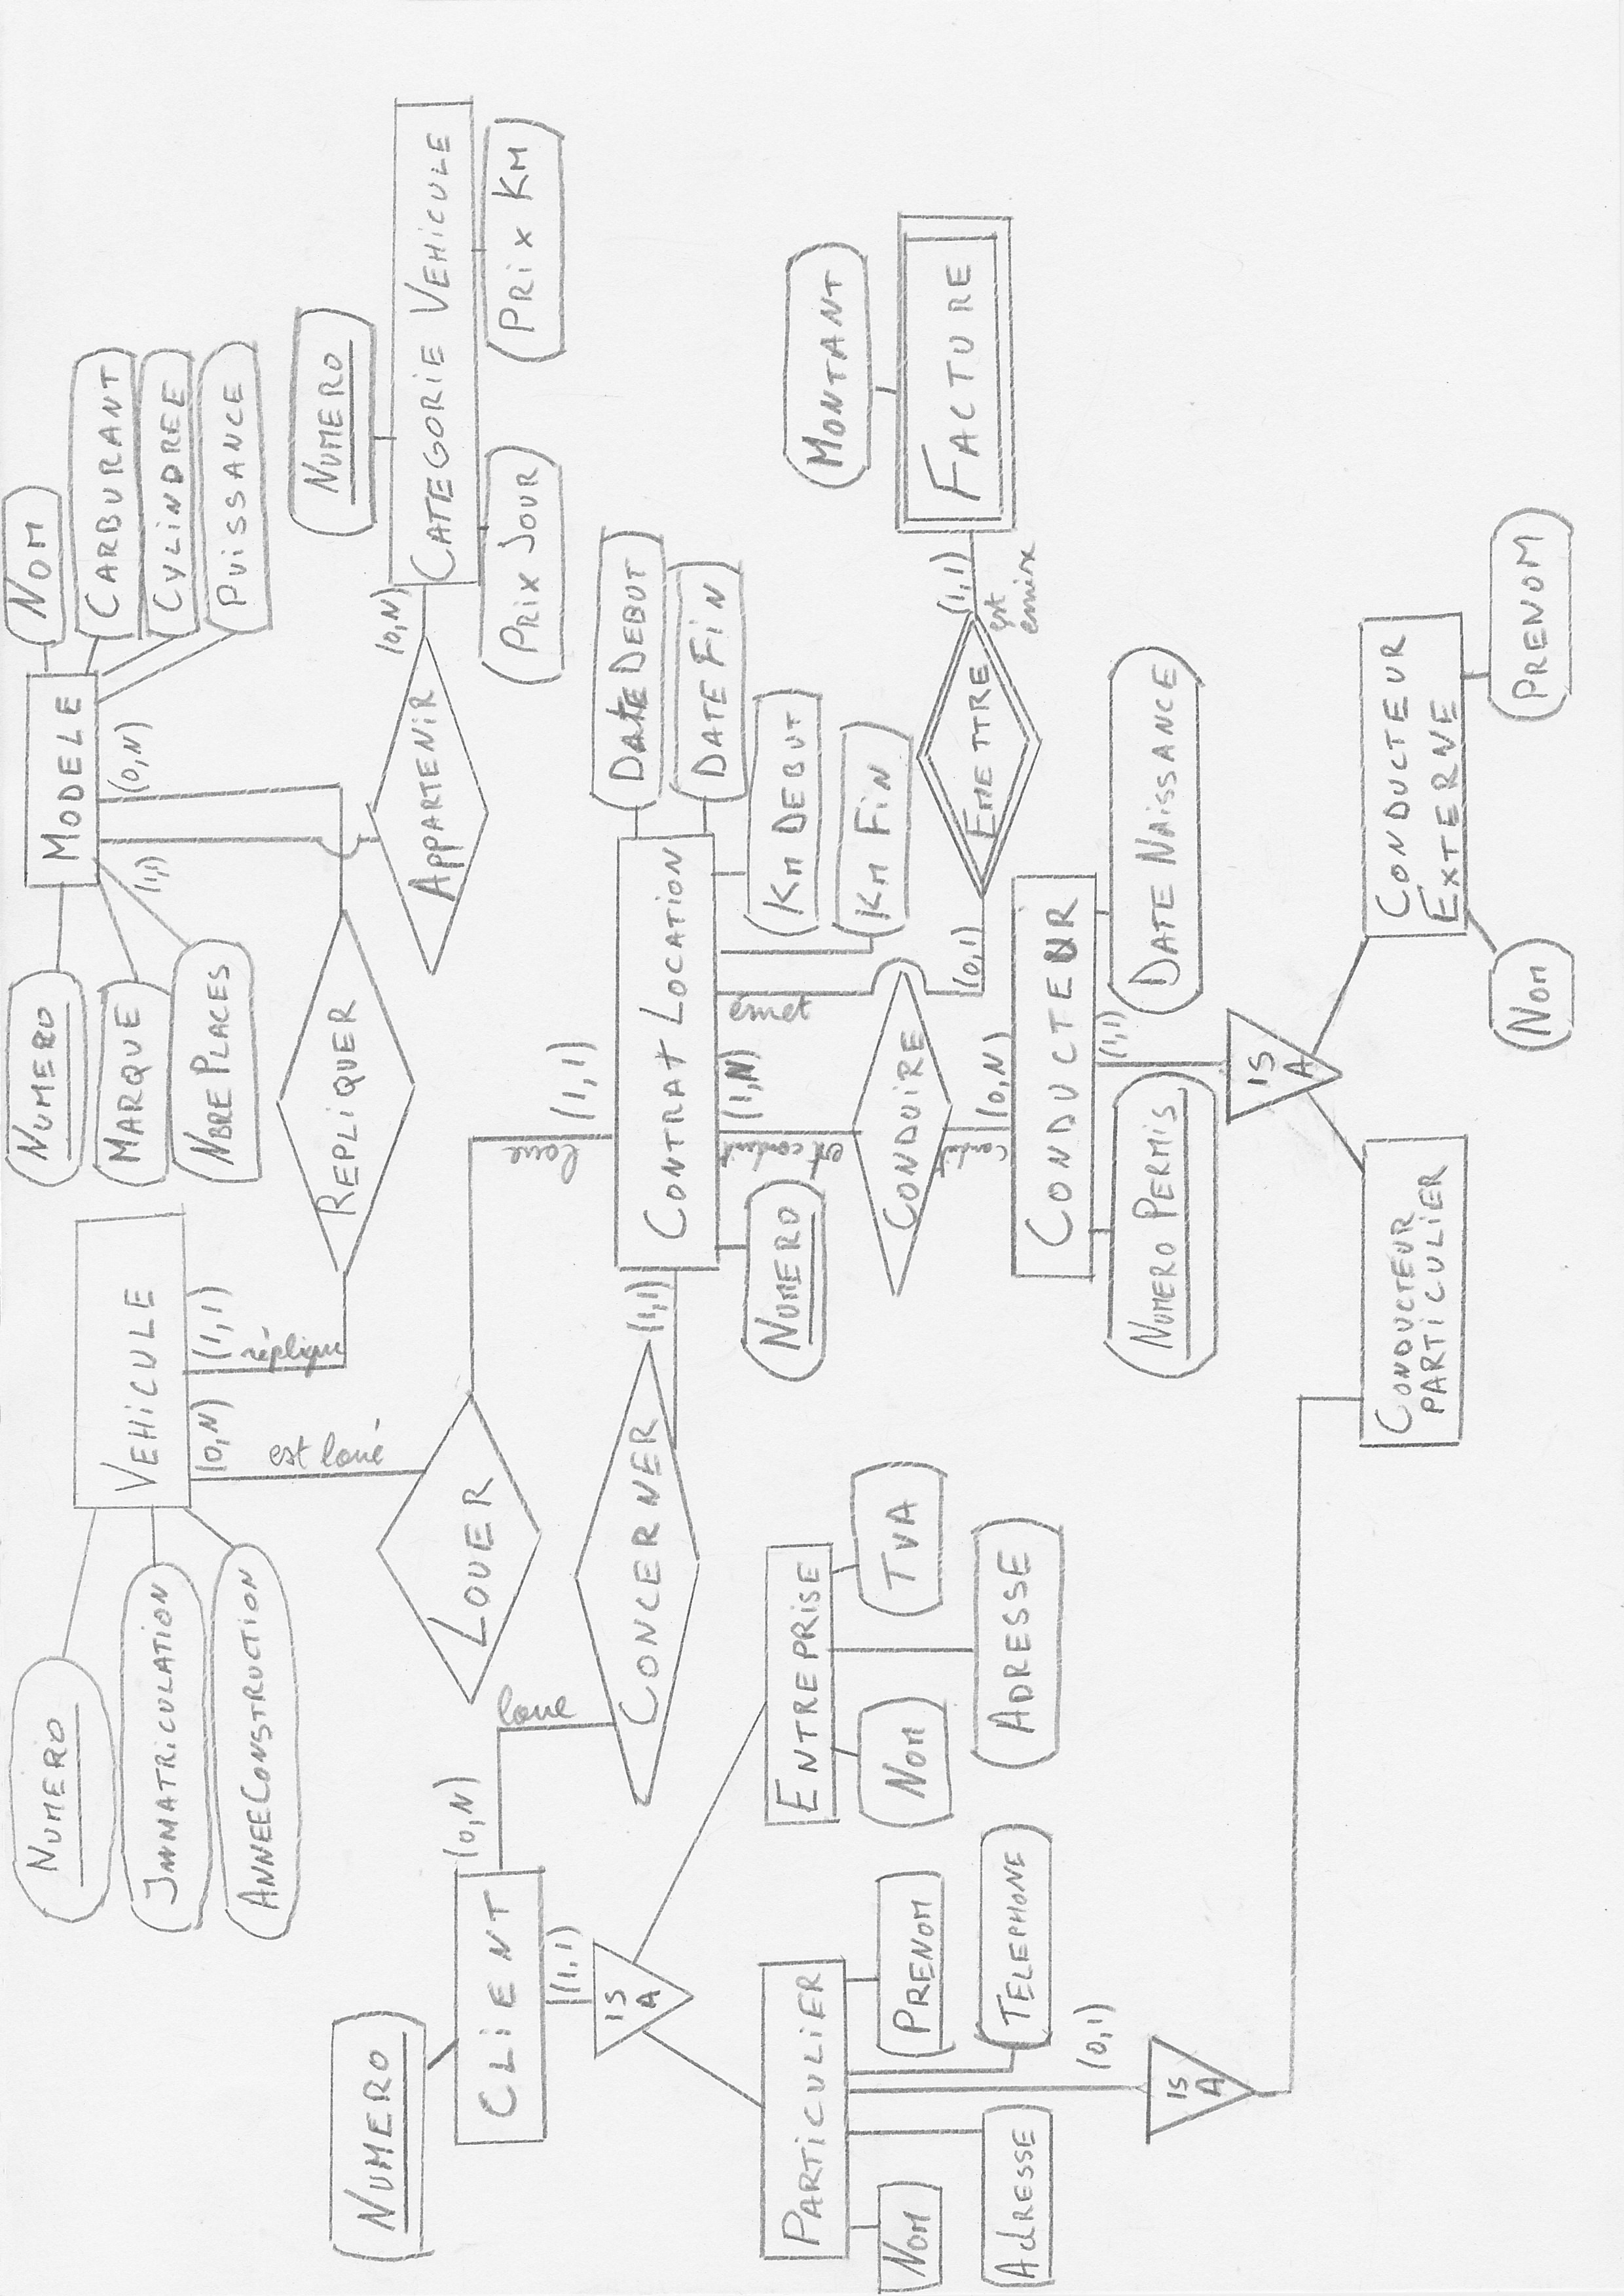
\includegraphics[width=\textwidth,height=\textheight]{modele.jpg}
    \label{diagramme}

\section{Modèle relationnel}

    \paragraph{}Les clé sont \underline{soulignées} et les clés étrangères sont
    \textit{en italique} avec le préfixe de la table référencée pour éviter 
    toute confusion.

    \paragraph{}
    \begin{itemize}
        \item \textbf{Véhicule}(\underline{Numéro}, Immatriculation,
        Année construction, \textit{Modèle.Numéro})
        \item \textbf{Modèle}(\underline{Numéro}, Marque, Nom, Nbre Places,
        Carburant, Cylindrée, Puissance, \textit{Catégorie Véhicule.Numéro})
        \item \textbf{Catégorie Véhicule}(\underline{Numéro}, Prix Jour,
        Prix Km)
    \end{itemize}

    \paragraph{}
    \begin{itemize}
        \item \textbf{Client}(\underline{Numéro})
        \item \textbf{Client Particulier}(\textit{\underline{Client.Numéro}},
        Nom, Prénom, Adresse, Téléphone)
        \item \textbf{Client Entreprise}(\textit{\underline{Client.Numéro}},
        Nom, TVA, Adresse)
    \end{itemize}

    \paragraph{}
    \begin{itemize}
        \item \textbf{Conducteur}(\underline{Numéro Permis}, Date Naissance)
        \item \textbf{Conducteur Particulier}(\textit{\underline{Conducteur.Numéro Permis}},
        \textit{Client.Numéro})
        \item \textbf{Conducteur Externe}(\textit{\underline{Conducteur.Numéro Permis}},
        Nom, Prénom)
    \end{itemize}

    \paragraph{}
    \begin{itemize}
        \item \textbf{Contrat Location}(\underline{Numéro}, Date Début, 
        Date Fin, Km Début, Km Fin, \textit{Client.Numéro}, 
        \textit{Véhicule.Numéro})
        \item \textbf{Conduire}(\textit{\underline{Conducteur.Numéro Permis}}, 
        \textit{\underline{Contrat Location.Numéro}})
        \item \textbf{Facture}(\textit{\underline{Contrat Location.Numéro}}, 
        Montant)
    \end{itemize}

\section{Dépendances fonctionnelles et normalisation}

    \subsubsection{Véhicule}
    \begin{itemize}
        \item Numéro $\rightarrow$ Immatriculation, Année construction,
        Modèle.Numéro
    \end{itemize}

    La relation est en 4FN et en BCNF.

    \subsubsection{Modèle}
    \begin{itemize}
        \item Numéro $\rightarrow$ Marque, Nom, Nbre Places, Carburant,
        Cylindrée, Puissance, Catégorie Véhicule.Numéro
        \item Marque, Nom $\rightarrow$ Numéro, Nbre Places, Carburant 
        Cylindrée, Puissance, Catégorie Véhicule.Numéro
    \end{itemize}

    La relation est en 4FN et en BCNF.

    \subsubsection{Catégorie Véhicule}
    \begin{itemize}
        \item Numéro $\rightarrow$ Prix Jour, Prix Km
    \end{itemize}

    La relation est en 4FN et en BCNF.

    \subsubsection{Client}

    La relation est en 4FN et en BCNF.

    \subsubsection{Client Particulier}
    \begin{itemize}
        \item Client.Numéro $\rightarrow$ Nom, Prénom, Adresse, Téléphone
        \item Nom, Prénom $\rightarrow$ Client.Numéro, Adresse, Téléphone
    \end{itemize}

    La relation est en 4FN et en BCNF.

    \subsubsection{Client Entreprise}
    \begin{itemize}
        \item Client.Numéro $\rightarrow$ Nom, TVA, Adresse
        \item Nom $\rightarrow$ Client.Numéro, TVA, Adresse
        \item TVA $\rightarrow$ Client.Numéro, Nom, Adresse
    \end{itemize}

    La relation est en 4FN et en BCNF.

    \subsubsection{Conducteur}
    \begin{itemize}
        \item Numéro Permis $\rightarrow$ Date Naissance
    \end{itemize}

    La relation est en 4FN et en BCNF.

    \subsubsection{Conducteur Particulier}
    \begin{itemize}
        \item Conducteur.Numéro Permis $\rightarrow$ Client.Numéro
        \item Client.Numéro $\rightarrow$ Conducteur.Numéro Permis
    \end{itemize}

    La relation est en 4FN et en BCNF.

    \subsubsection{Conducteur Entreprise}
    \begin{itemize}
        \item Conducteur.Numéro Permis $\rightarrow$ Client.Numéro
        \item Client.Numéro $\rightarrow$ Conducteur.Numéro Permis
    \end{itemize}

    La relation est en 4FN et en BCNF.

    \subsubsection{Contrat Location}
    \begin{itemize}
        \item Numéro $\rightarrow$ Date Début, Date Fin, Km Début, Km Fin,
        Client.Numéro, Véhicule.Numéro
        \item Date Début, Date Fin, Véhicule.Numéro $\rightarrow$ Numéro,
        Km Début, Km Fin, Client.Numéro
        \item Km Début, Km Fin, Véhicule.Numéro $\rightarrow$ Numéro,
        Date Début, Date Fin, Client.Numéro
    \end{itemize}

    La relation est en 4FN et en BCNF.

    \subsubsection{Conduire}
    \begin{itemize}
        \item Conducteur.Numéro Permis $\rightarrow\rightarrow$
        Contrat Location.Numéro
        \item Contrat Location.Numéro $\rightarrow\rightarrow$
        Conducteur.Numéro Permis
    \end{itemize}

    La relation est en 4FN et en BCNF.

    \subsubsection{Facture}
    \begin{itemize}
        \item Contrat Location.Numéro $\rightarrow$ Montant
    \end{itemize}

    La relation est en 4FN et en BCNF.

\end{changemargin}
\end{document}